\section{Introduction}

\begin{definition}[\textit{Data Base Management System}]
    A Database Management System (DBMS) is a software product designed to manage collections of data that possess the following characteristics:
    \begin{itemize}
        \item \textit{Large}: the data collections are significantly larger than the central memory available on the computers that run the software.
        \item \textit{Persistent}: the data has a lifespan independent of individual executions of the programs that access it.
        \item \textit{Shared}: the data is accessed by multiple applications simultaneously.
        \item \textit{Reliable}: the system ensures tolerance to hardware and software failures.
        \item \textit{Respectful of Data Ownership}: access is disciplined and controlled.
    \end{itemize}
\end{definition}

Key developments in DBMS technology are outlined in the following chronological timeline:

\begin{chronology}[5]{1990}{2020}{0.9\textwidth}
    \event{1992}{SQL '92}
    \event{1999}{SQL '99}
    \event{2001}{Ranking in databases}
    \event{2003}{XML-related features}
    \event{2005}{NoSQL}
    \event{2006}{X-Query}
    \event{2009}{JPA final release}
    \event{2011}{Temporal databases}
    \event{2016}{JSON}
\end{chronology}

The architecture of a DBMS is illustrated in the figure below:
\begin{figure}[H]
    \centering
    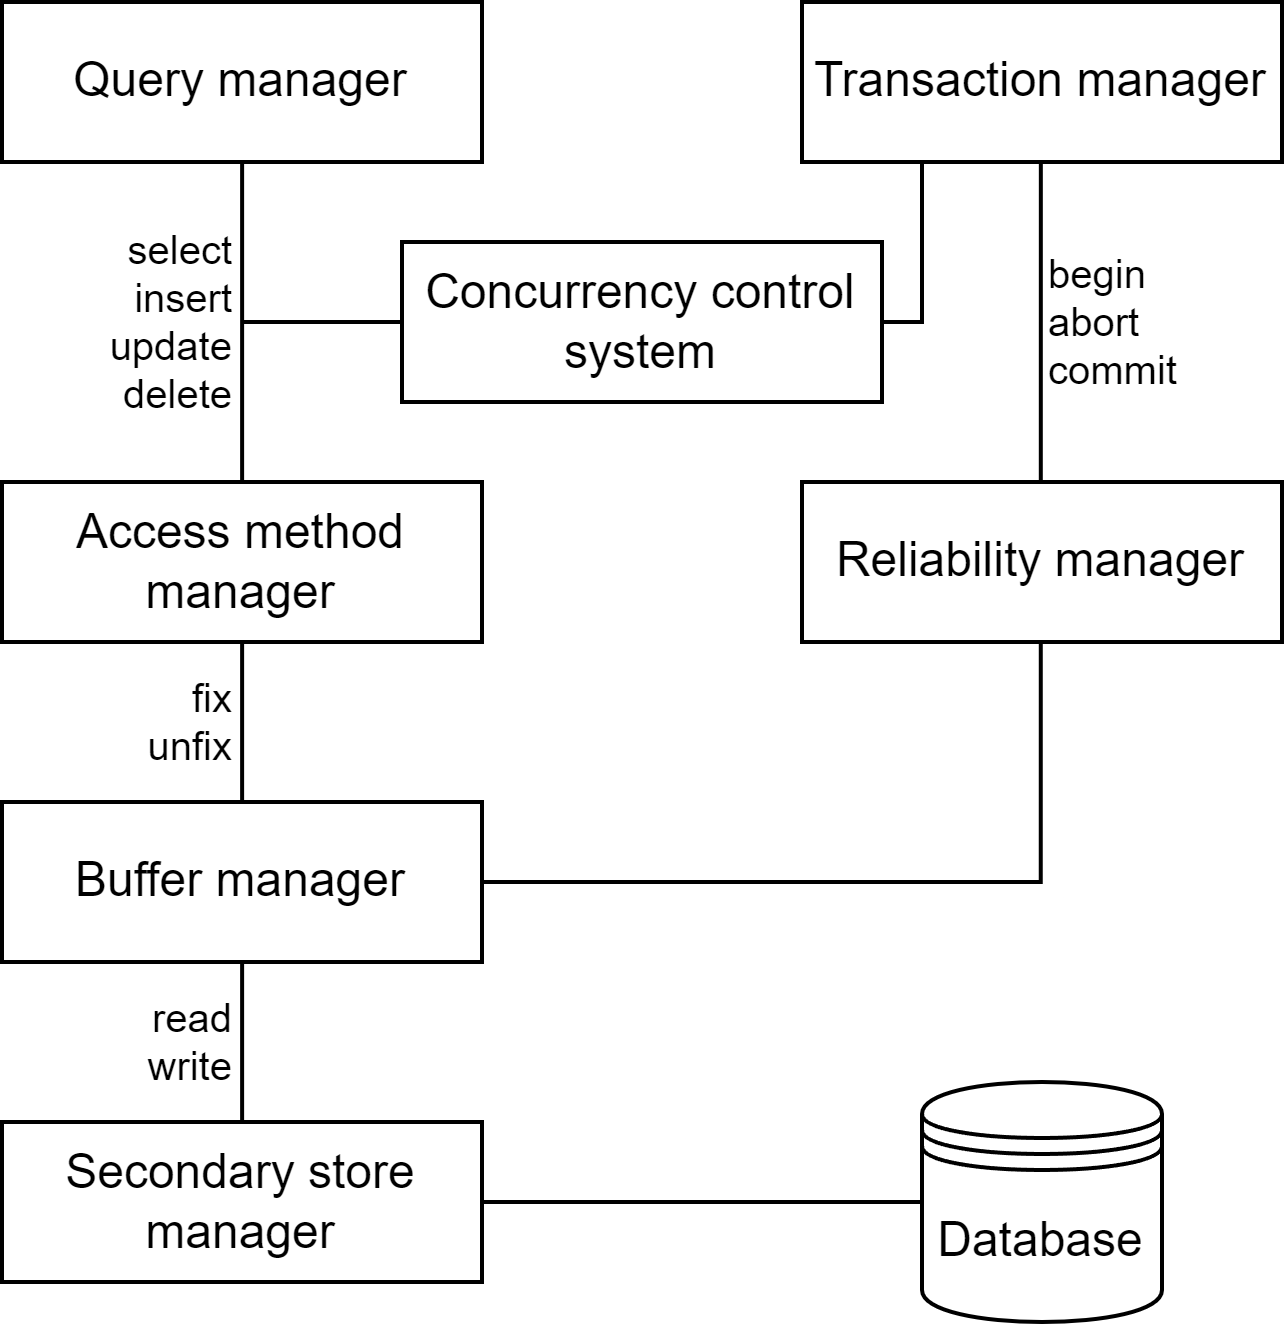
\includegraphics[width=0.5\linewidth]{images/architecture.png}
    \caption{DBMS architecture}
\end{figure}